% GENERATED by bin/curate/gen_sdem_validation.py from the engine and
% tutorials/steady/membranes/membrane12_sdem_nf270_nacl_traces/constant/experimental/fdl2021_figures.csv
% -- do not edit; regenerate.  Checked for drift by the same script with --check.
\begin{figure}[htbp]
\centering
\definecolor{sdemNa}{HTML}{0072B2}
\definecolor{sdemMg}{HTML}{E69F00}
\definecolor{sdemNH4}{HTML}{009E73}
\definecolor{sdemCl}{HTML}{D55E00}
\definecolor{sdemNO3}{HTML}{CC79A7}
\definecolor{sdemSO4}{HTML}{000000}
\pgfplotsset{sdempanel/.style={width=0.5\textwidth, height=0.4\textwidth, log ticks with fixed point, xlabel={$J_v$ ($\mu$m/s)}, ylabel={$f = 1/(1-R)$}, xmin=0, grid=major, grid style={gray!20}, tick label style={font=\scriptsize}, label style={font=\scriptsize}, title style={font=\footnotesize}, legend style={font=\scriptsize, at={(0.5,-0.24)}, anchor=north, draw=none, legend columns=3, /tikz/every even column/.append style={column sep=6pt}}, legend cell align=left}}
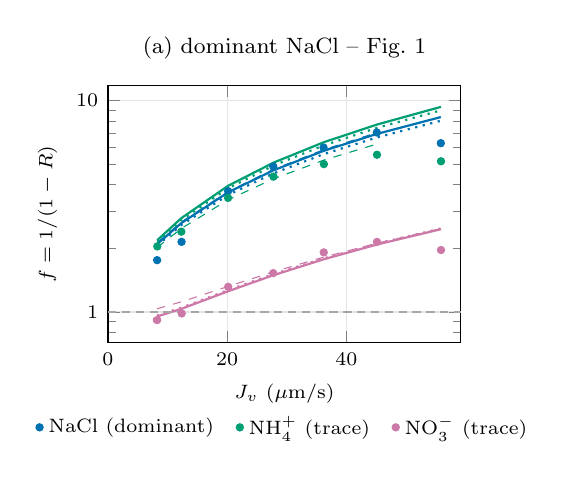
\begin{tikzpicture}\begin{semilogyaxis}[sdempanel, xmax=59.2, title={(a) dominant NaCl -- Fig.~1}]
\addplot[sdemNa, only marks, mark=*, mark size=1.3pt, error bars/.cd, y dir=both, y explicit] coordinates {(8.24,1.7579) +- (0,0.0168) (12.34,2.1449) +- (0,0.0168) (20.15,3.7262) +- (0,0.0168) (27.73,4.8701) +- (0,0.0168) (36.17,5.9804) +- (0,0.0168) (45.10,7.0486) +- (0,0.0168) (55.84,6.2748) +- (0,0.0168)}; \addlegendentry{NaCl (dominant)}
\addplot[sdemNa, dashed, thin, forget plot] coordinates {(8.24,2.1208) (12.34,2.6660) (20.15,3.7064) (27.73,4.7152) (36.17,5.8406) (45.10,7.0320)};
\addplot[sdemNa, solid, thick, forget plot] coordinates {(8.24,2.0919) (12.34,2.6360) (20.15,3.6767) (27.73,4.6680) (36.17,5.7721) (45.10,6.9379) (55.84,8.3361)};
\addplot[sdemNa, dotted, thick, forget plot] coordinates {(8.24,2.0597) (12.34,2.5806) (20.15,3.5728) (27.73,4.5164) (36.17,5.5669) (45.10,6.6764) (55.84,8.0071)};
\addplot[sdemNH4, only marks, mark=*, mark size=1.3pt, error bars/.cd, y dir=both, y explicit] coordinates {(8.27,2.0405) +- (0,0.0156) (12.30,2.3956) +- (0,0.0125) (20.14,3.4611) +- (0,0.0125) (27.76,4.3614) +- (0,0.0125) (36.22,4.9969) +- (0,0.0218) (45.13,5.5327) +- (0,0.0218) (55.87,5.1526) +- (0,0.0218)}; \addlegendentry{NH$_4^+$ (trace)}
\addplot[sdemNH4, dashed, thin, forget plot] coordinates {(8.27,2.0197) (12.30,2.4810) (20.14,3.3879) (27.76,4.2596) (36.22,5.2196) (45.13,6.2192)};
\addplot[sdemNH4, solid, thick, forget plot] coordinates {(8.27,2.1847) (12.30,2.7751) (20.14,3.9454) (27.76,5.0761) (36.22,6.3426) (45.13,7.6866) (55.87,9.3147)};
\addplot[sdemNH4, dotted, thick, forget plot] coordinates {(8.27,2.1518) (12.30,2.7187) (20.14,3.8384) (27.76,4.9188) (36.22,6.1290) (45.13,7.4136) (55.87,8.9703)};
\addplot[sdemNO3, only marks, mark=*, mark size=1.3pt, error bars/.cd, y dir=both, y explicit] coordinates {(8.23,0.9159) +- (0,0.0125) (12.37,0.9844) +- (0,0.0125) (20.16,1.3146) +- (0,0.0125) (27.71,1.5265) +- (0,0.0125) (36.20,1.9128) +- (0,0.0125) (45.13,2.1433) +- (0,0.0125) (55.87,1.9626) +- (0,0.0125)}; \addlegendentry{NO$_3^-$ (trace)}
\addplot[sdemNO3, dashed, thin, forget plot] coordinates {(8.23,1.0362) (12.37,1.1182) (20.16,1.3209) (27.71,1.5474) (36.20,1.8172) (45.13,2.1132) (55.87,2.4770)};
\addplot[sdemNO3, solid, thick, forget plot] coordinates {(8.23,0.9516) (12.37,1.0364) (20.16,1.2533) (27.71,1.4910) (36.20,1.7749) (45.13,2.0834) (55.87,2.4613)};
\addplot[sdemNO3, dotted, thick, forget plot] coordinates {(8.23,0.9621) (12.37,1.0495) (20.16,1.2692) (27.71,1.5082) (36.20,1.7932) (45.13,2.1024) (55.87,2.4812)};
\addplot[gray!70, densely dashed, thin, forget plot] coordinates {(0,1) (59.2,1)};
\end{semilogyaxis}\end{tikzpicture}\hfill
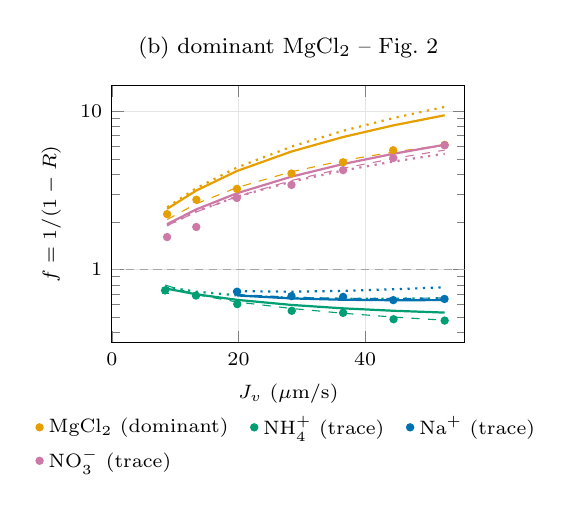
\begin{tikzpicture}\begin{semilogyaxis}[sdempanel, xmax=55.7, title={(b) dominant MgCl$_2$ -- Fig.~2}]
\addplot[sdemMg, only marks, mark=*, mark size=1.3pt, error bars/.cd, y dir=both, y explicit] coordinates {(8.73,2.2368) +- (0,0.0132) (13.35,2.7566) +- (0,0.0132) (19.75,3.2303) +- (0,0.0132) (28.36,4.0395) +- (0,0.0132) (36.49,4.7566) +- (0,0.0132) (44.41,5.6645) +- (0,0.0132) (52.54,6.1250) +- (0,0.0132)}; \addlegendentry{MgCl$_2$ (dominant)}
\addplot[sdemMg, dashed, thin, forget plot] coordinates {(8.73,2.0684) (13.35,2.6033) (19.75,3.2918) (28.36,4.1431) (36.49,4.8742) (44.41,5.5199) (52.54,6.1205)};
\addplot[sdemMg, solid, thick, forget plot] coordinates {(8.73,2.4158) (13.35,3.1562) (19.75,4.1885) (28.36,5.5624) (36.49,6.8653) (44.41,8.1293) (52.54,9.4221)};
\addplot[sdemMg, dotted, thick, forget plot] coordinates {(8.73,2.4711) (13.35,3.2674) (19.75,4.4075) (28.36,5.9750) (36.49,7.5118) (44.41,9.0434) (52.54,10.6483)};
\addplot[sdemNH4, only marks, mark=*, mark size=1.3pt, error bars/.cd, y dir=both, y explicit] coordinates {(8.41,0.7381) +- (0,0.0292) (13.28,0.6845) +- (0,0.0059) (19.80,0.6041) +- (0,0.0052) (28.40,0.5483) +- (0,0.0047) (36.51,0.5320) +- (0,0.0081) (44.47,0.4849) +- (0,0.0042) (52.54,0.4756) +- (0,0.0052)}; \addlegendentry{NH$_4^+$ (trace)}
\addplot[sdemNH4, dashed, thin, forget plot] coordinates {(8.41,0.7977) (13.28,0.6942) (19.80,0.6230) (28.40,0.5669) (36.51,0.5290) (44.47,0.5004) (52.54,0.4782)};
\addplot[sdemNH4, solid, thick, forget plot] coordinates {(8.41,0.7601) (13.28,0.6977) (19.80,0.6427) (28.40,0.5969) (36.51,0.5682) (44.47,0.5485) (52.54,0.5342)};
\addplot[sdemNH4, dotted, thick, forget plot] coordinates {(8.41,0.7758) (13.28,0.7248) (19.80,0.6863) (28.40,0.6623) (36.51,0.6541) (44.47,0.6538) (52.54,0.6584)};
\addplot[sdemNa, only marks, mark=*, mark size=1.3pt, error bars/.cd, y dir=both, y explicit] coordinates {(19.77,0.7239) +- (0,0.0078) (28.36,0.6786) +- (0,0.0059) (36.51,0.6713) +- (0,0.0058) (44.43,0.6403) +- (0,0.0055) (52.52,0.6514) +- (0,0.0056)}; \addlegendentry{Na$^+$ (trace)}
\addplot[sdemNa, dashed, thin, forget plot] coordinates {(19.77,0.6951) (28.36,0.6682) (36.51,0.6570) (44.43,0.6559) (52.52,0.6606)};
\addplot[sdemNa, solid, thick, forget plot] coordinates {(19.77,0.6854) (28.36,0.6565) (36.51,0.6437) (44.43,0.6395) (52.52,0.6407)};
\addplot[sdemNa, dotted, thick, forget plot] coordinates {(19.77,0.7299) (28.36,0.7239) (36.51,0.7331) (44.43,0.7498) (52.52,0.7719)};
\addplot[sdemNO3, only marks, mark=*, mark size=1.3pt, error bars/.cd, y dir=both, y explicit] coordinates {(8.72,1.6027) +- (0,0.0139) (13.33,1.8556) +- (0,0.0161) (19.73,2.8302) +- (0,0.0245) (28.36,3.4209) +- (0,0.0296) (36.51,4.2432) +- (0,0.0367) (44.43,5.0629) +- (0,0.0438) (52.54,6.0932) +- (0,0.0527)}; \addlegendentry{NO$_3^-$ (trace)}
\addplot[sdemNO3, dashed, thin, forget plot] coordinates {(8.72,1.8913) (13.33,2.3090) (19.73,2.8869) (28.36,3.6496) (36.51,4.3541) (44.43,5.0249) (52.54,5.6740)};
\addplot[sdemNO3, solid, thick, forget plot] coordinates {(8.72,1.9331) (13.33,2.3962) (19.73,3.0293) (28.36,3.8589) (36.51,4.6356) (44.43,5.3806) (52.54,6.1356)};
\addplot[sdemNO3, dotted, thick, forget plot] coordinates {(8.72,1.8986) (13.33,2.3245) (19.73,2.8859) (28.36,3.5889) (36.51,4.2200) (44.43,4.8051) (52.54,5.3818)};
\addplot[gray!70, densely dashed, thin, forget plot] coordinates {(0,1) (55.7,1)};
\end{semilogyaxis}\end{tikzpicture}\\[18pt]
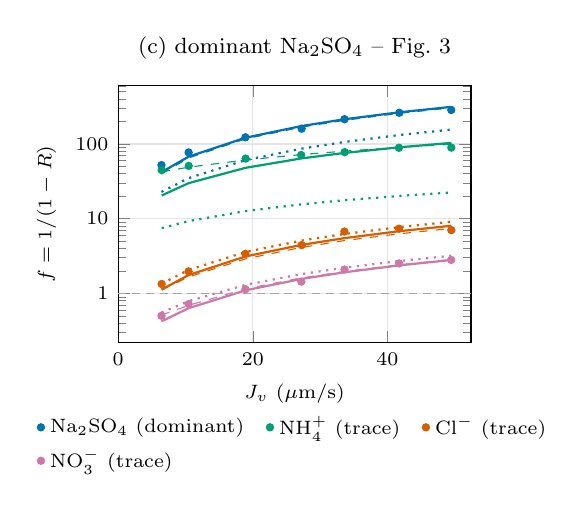
\begin{tikzpicture}\begin{semilogyaxis}[sdempanel, xmax=52.4, title={(c) dominant Na$_2$SO$_4$ -- Fig.~3}]
\addplot[sdemNa, only marks, mark=*, mark size=1.3pt, error bars/.cd, y dir=both, y explicit] coordinates {(6.43,52.2045) +- (0,0.6567) (10.47,77.1576) +- (0,0.6567) (18.90,122.7955) +- (0,0.6567) (27.25,160.2251) +- (0,0.6567) (33.62,214.7280) +- (0,0.6567) (41.76,261.6792) +- (0,0.6567) (49.47,284.9906) +- (0,0.6567)}; \addlegendentry{Na$_2$SO$_4$ (dominant)}
\addplot[sdemNa, dashed, thin, forget plot] coordinates {(6.43,39.7887) (10.47,65.0774) (18.90,116.9960) (27.25,168.3799) (33.62,207.3400) (41.76,257.3438) (49.47,304.6724)};
\addplot[sdemNa, solid, thick, forget plot] coordinates {(6.43,41.9884) (10.47,67.5879) (18.90,121.1874) (27.25,174.0242) (33.62,214.2539) (41.76,265.4958) (49.47,313.9624)};
\addplot[sdemNa, dotted, thick, forget plot] coordinates {(6.43,22.8314) (10.47,34.9334) (18.90,60.7798) (27.25,86.6052) (33.62,106.4277) (41.76,131.8277) (49.47,155.9798)};
\addplot[sdemNH4, only marks, mark=*, mark size=1.3pt, error bars/.cd, y dir=both, y explicit] coordinates {(6.46,44.7539) +- (0,0.2321) (10.48,50.8821) +- (0,0.2321) (18.93,63.7883) +- (0,0.3250) (27.18,71.2163) +- (0,0.1857) (33.64,77.8087) +- (0,0.3250) (41.70,88.9508) +- (0,0.1857) (49.48,89.4615) +- (0,0.2786)}; \addlegendentry{NH$_4^+$ (trace)}
\addplot[sdemNH4, dashed, thin, forget plot] coordinates {(6.46,42.5388) (10.48,48.8789) (18.93,61.1173) (27.18,72.0979) (33.64,80.2589) (41.70,90.0217) (49.48,99.1020)};
\addplot[sdemNH4, solid, thick, forget plot] coordinates {(6.46,20.4410) (10.48,29.9402) (18.93,47.9728) (27.18,64.0442) (33.64,75.9544) (41.70,90.1897) (49.48,103.3910)};
\addplot[sdemNH4, dotted, thick, forget plot] coordinates {(6.46,7.4753) (10.48,9.2903) (18.93,12.6500) (27.18,15.5580) (33.64,17.6679) (41.70,20.1459) (49.48,22.4064)};
\addplot[sdemCl, only marks, mark=*, mark size=1.3pt, error bars/.cd, y dir=both, y explicit] coordinates {(6.46,1.3370) +- (0,0.0334) (10.47,1.9721) +- (0,0.0334) (18.90,3.3844) +- (0,0.0334) (27.25,4.4290) +- (0,0.0334) (33.60,6.7354) +- (0,0.0334) (41.72,7.3538) +- (0,0.0334) (49.48,7.0362) +- (0,0.0334)}; \addlegendentry{Cl$^-$ (trace)}
\addplot[sdemCl, dashed, thin, forget plot] coordinates {(6.46,1.1129) (10.47,1.6626) (18.90,2.8958) (27.25,4.1304) (33.60,5.0938) (41.72,6.2740) (49.48,7.4220)};
\addplot[sdemCl, solid, thick, forget plot] coordinates {(6.46,1.1268) (10.47,1.7610) (18.90,3.1188) (27.25,4.4666) (33.60,5.4903) (41.72,6.7961) (49.48,8.0404)};
\addplot[sdemCl, dotted, thick, forget plot] coordinates {(6.46,1.3494) (10.47,2.0614) (18.90,3.5868) (27.25,5.0976) (33.60,6.2439) (41.72,7.7049) (49.48,9.0960)};
\addplot[sdemNO3, only marks, mark=*, mark size=1.3pt, error bars/.cd, y dir=both, y explicit] coordinates {(6.44,0.5014) +- (0,0.0334) (10.47,0.7187) +- (0,0.0334) (18.90,1.1365) +- (0,0.0334) (27.21,1.4373) +- (0,0.0334) (33.62,2.0891) +- (0,0.0334) (41.74,2.5237) +- (0,0.0334) (49.46,2.8078) +- (0,0.0334)}; \addlegendentry{NO$_3^-$ (trace)}
\addplot[sdemNO3, dashed, thin, forget plot] coordinates {(6.44,0.5141) (10.47,0.6915) (18.90,1.1492) (27.21,1.6127) (33.62,1.9654) (41.74,2.4182) (49.46,2.8422)};
\addplot[sdemNO3, solid, thick, forget plot] coordinates {(6.44,0.4229) (10.47,0.6341) (18.90,1.0979) (27.21,1.5609) (33.62,1.9183) (41.74,2.3708) (49.46,2.8004)};
\addplot[sdemNO3, dotted, thick, forget plot] coordinates {(6.44,0.5565) (10.47,0.7881) (18.90,1.2995) (27.21,1.8125) (33.62,2.2093) (41.74,2.7124) (49.46,3.1903)};
\addplot[gray!70, densely dashed, thin, forget plot] coordinates {(0,1) (52.4,1)};
\end{semilogyaxis}\end{tikzpicture}\hfill
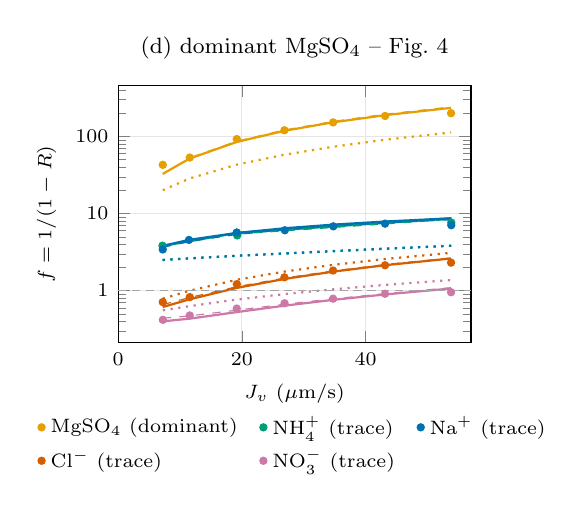
\begin{tikzpicture}\begin{semilogyaxis}[sdempanel, xmax=57.0, title={(d) dominant MgSO$_4$ -- Fig.~4}]
\addplot[sdemMg, only marks, mark=*, mark size=1.3pt, error bars/.cd, y dir=both, y explicit] coordinates {(7.21,42.9174) +- (0,0.5629) (11.57,53.3302) +- (0,0.5629) (19.17,92.5891) +- (0,0.5629) (26.86,120.4503) +- (0,0.5629) (34.73,152.2514) +- (0,0.5629) (43.13,184.3340) +- (0,0.5629) (53.78,200.5159) +- (0,0.5629)}; \addlegendentry{MgSO$_4$ (dominant)}
\addplot[sdemMg, dashed, thin, forget plot] coordinates {(7.21,32.5806) (11.57,52.9156) (19.17,87.0073) (26.86,121.6265) (34.73,157.0052) (43.13,194.7833) (53.78,242.2365)};
\addplot[sdemMg, solid, thick, forget plot] coordinates {(7.21,32.7519) (11.57,51.8177) (19.17,84.9762) (26.86,118.4519) (34.73,152.6235) (43.13,189.0322) (53.78,235.0071)};
\addplot[sdemMg, dotted, thick, forget plot] coordinates {(7.21,20.1004) (11.57,28.6245) (19.17,43.1359) (26.86,58.0067) (34.73,73.5940) (43.13,90.6888) (53.78,112.9751)};
\addplot[sdemNH4, only marks, mark=*, mark size=1.3pt, error bars/.cd, y dir=both, y explicit] coordinates {(7.16,3.8380) +- (0,0.0461) (19.23,5.2123) +- (0,0.0209) (53.82,7.6508) +- (0,0.0293)}; \addlegendentry{NH$_4^+$ (trace)}
\addplot[sdemNH4, dashed, thin, forget plot] coordinates {(19.23,5.4291) (53.82,8.4158)};
\addplot[sdemNH4, solid, thick, forget plot] coordinates {(7.16,3.8036) (19.23,5.6183) (53.82,8.6857)};
\addplot[sdemNH4, dotted, thick, forget plot] coordinates {(7.16,2.5031) (19.23,2.8377) (53.82,3.8251)};
\addplot[sdemNa, only marks, mark=*, mark size=1.3pt, error bars/.cd, y dir=both, y explicit] coordinates {(7.21,3.4274) +- (0,0.0168) (11.44,4.5545) +- (0,0.0335) (19.16,5.6983) +- (0,0.0168) (26.93,6.0796) +- (0,0.0251) (34.76,6.8380) +- (0,0.0838) (43.12,7.4078) +- (0,0.0168) (53.82,7.0726) +- (0,0.0168)}; \addlegendentry{Na$^+$ (trace)}
\addplot[sdemNa, dashed, thin, forget plot] coordinates {(7.21,3.6434) (11.44,4.3447) (19.16,5.3582) (26.93,6.1608) (34.76,6.8976) (43.12,7.5433) (53.82,8.3165)};
\addplot[sdemNa, solid, thick, forget plot] coordinates {(7.21,3.8149) (11.44,4.5625) (19.16,5.6129) (26.93,6.4593) (34.76,7.1937) (43.12,7.8914) (53.82,8.6935)};
\addplot[sdemNa, dotted, thick, forget plot] coordinates {(7.21,2.5058) (11.44,2.6339) (19.16,2.8382) (26.93,3.0495) (34.76,3.2714) (43.12,3.5148) (53.82,3.8316)};
\addplot[sdemCl, only marks, mark=*, mark size=1.3pt, error bars/.cd, y dir=both, y explicit] coordinates {(7.21,0.7123) +- (0,0.0335) (11.57,0.8254) +- (0,0.0168) (19.18,1.2151) +- (0,0.0168) (26.86,1.4916) +- (0,0.0168) (34.72,1.8268) +- (0,0.0168) (43.12,2.1369) +- (0,0.0168) (53.78,2.3128) +- (0,0.0168)}; \addlegendentry{Cl$^-$ (trace)}
\addplot[sdemCl, dashed, thin, forget plot] coordinates {(7.21,0.6598) (11.57,0.8173) (19.18,1.1270) (26.86,1.4590) (34.72,1.8074) (43.12,2.1850) (53.78,2.6649)};
\addplot[sdemCl, solid, thick, forget plot] coordinates {(7.21,0.6149) (11.57,0.7744) (19.18,1.0879) (26.86,1.4202) (34.72,1.7671) (43.12,2.1410) (53.78,2.6179)};
\addplot[sdemCl, dotted, thick, forget plot] coordinates {(7.21,0.7876) (11.57,1.0026) (19.18,1.3858) (26.86,1.7711) (34.72,2.1626) (43.12,2.5770) (53.78,3.0987)};
\addplot[sdemNO3, only marks, mark=*, mark size=1.3pt, error bars/.cd, y dir=both, y explicit] coordinates {(7.23,0.4190) +- (0,0.0168) (11.57,0.4777) +- (0,0.0168) (19.16,0.5866) +- (0,0.0168) (26.88,0.6872) +- (0,0.0168) (34.72,0.7877) +- (0,0.0168) (43.12,0.9134) +- (0,0.0168) (53.78,0.9553) +- (0,0.0168)}; \addlegendentry{NO$_3^-$ (trace)}
\addplot[sdemNO3, dashed, thin, forget plot] coordinates {(7.23,0.4398) (11.57,0.4714) (19.16,0.5595) (26.88,0.6676) (34.72,0.7854) (43.12,0.9165) (53.78,1.0963)};
\addplot[sdemNO3, solid, thick, forget plot] coordinates {(7.23,0.4007) (11.57,0.4341) (19.16,0.5279) (26.88,0.6397) (34.72,0.7607) (43.12,0.8942) (53.78,1.0671)};
\addplot[sdemNO3, dotted, thick, forget plot] coordinates {(7.23,0.5576) (11.57,0.6314) (19.16,0.7669) (26.88,0.9040) (34.72,1.0422) (43.12,1.1890) (53.78,1.3744)};
\addplot[gray!70, densely dashed, thin, forget plot] coordinates {(0,1) (57.0,1)};
\end{semilogyaxis}\end{tikzpicture}
\caption{Choupo against the paper, every digitised point of Figures 1--4.  $f = 1/(1-R)$ on a log axis; below the grey line ($f = 1$) a rejection is negative.  Markers: the measured points, the bar being the reading error of the digitisation; dashed: the paper's fitted line (Eq.~(1) for the salt, Eq.~(3) for a trace); solid: Choupo at the same flux in the trace limit (trace salts at $2\times10^{-7}$~mol/L); dotted: Choupo at the paper's feed ($2\times10^{-4}$~mol/L).  The dominant salt is drawn through its cation; in the trace limit its two ions coincide exactly.  One colour per ion across the four panels.}
\label{fig:sdem-validation}
\end{figure}
